\subsection*{Experimental setup}
In order to perform the experimental evaluation we used a tool to automatically
detect sentiment shift in tweets coming from year 2009 and regarding several
topics. We also downloaded news from the \emph{New York Times} and \emph{ABC
Australia} on the same topic and spanning on the same period of the tweets.

It's important to remember that tweet have different language structure that need to be normalized, so for cleaning purpose, the following operations were performed on the tweet text before starting the computation of all the different methodologies:
\begin{itemize}
	\item URLs removal from tweets using a regular expression
	\item conversion from Unicode to ASCII
\end{itemize}

In addition, while parsing the news, we considered the possibility that the
opinion expressed by tweets might be both delayed or in advance with respect to
news (e.g. if a movie becomes popular it is probable that news spread very fast
on twitter, but slower on newspaper, whereas other topics are discussed on
twitter only after news about them came out for several days). Thus, we
considered a enlarged time window for news which starts 5 days before the
beginning of the contradiction and last up to 5 days after the end of it.

After that, we manually labelled each contradiction point with the event which
caused it. The topics, contradiction points and events used for the experiments
are showed in table \ref{tab:setup}

\begin{table*}
	\centering
	\begin{tabularx}{\textwidth}{|l|l|X|}
	\hline
	Contr. point 	& Contr. window 			& Event \\
	\hline 
	Cern1			& 2009-10-29 - 2009-11-08 	& On November 3rd a bird drops a
piece of bread which cause LHC overheating. \\
	Cern2			& 2009-11-24 - 2009-12-04	& On November 30th LHC accelerates protons to an
energy of 1.18 TeV, becoming the world most powerful energy particle
accelerator\\
	FortHood 		& 2009-11-02 - 2009-11-06	& On November 5th a US marine
kills 13 people\\
	HangOver		& 2009-06-21 - 2009-06-27	& undetermined or movie released
	on June 5th\\
	Lcross			& 2009-10-31 - 2009-11-08	& Preliminary findings from
	Lcross. Others announced\\
	Jackson1		& 2009-06-19 - 2009-06-25	& On June 25th Michael Jackson
dies\\
	Jackson2		& 2009-08-23 - 2009-08-29	& On august 28th another popular
musician, Adam Goldstein, dies. The day after, August 29th is Jackson's
birthday\\
	SwineFlu		& 2009-06-19 - 2009-06-23	& The swine flu is recognized as
	a pandemic\\
	\hline
	\end{tabularx}
	\caption{Contradiction points used for experimental evaluation}
	\label{tab:setup}
\end{table*}

\subsection*{Experiments}
\subsubsection*{SpaceSaving evaluation}
The results achieved using the \emph{SpaceSaving} methodology with a maximum
error of five days on the contradiction window are shown in table
\ref{tab:resultsSS}.
\subsubsection*{Description of the algorithm}
\emph{SpaceSaving} \cite{SS} is an algorithm which was first presented by Metwally et al.
in 2005 to efficiently compute the most frequent terms in a data stream. It
allows the user to find $k$ words which are among the most frequent in the given
stream. Although this is a heuristic algorithm whose result's correctness is not
guaranteed, SpaceSaving is able to specify the upper bound of the error for each
word presented as output.

The classic implementation is based on a fixed size list of tuple 
\begin{displaymath}
	(word, occurrencies, error)
\end{displaymath}
The stream is read word by word and at any time one of the following condition
is verified:
\begin{enumerate}
	\item \label{SS-among-frequent}
		the word is already in the list of frequent terms
	\item \label{SS-list-not-full}
		the word is not among the frequent terms, but the list is not full
	\item \label{SS-list-full}
		the word is not among the frequent terms and the list is full
\end{enumerate}
If the first condition is verified, then the algorithm will proceed incrementing
the number of occurrencies of that term; if condition \ref{SS-list-not-full} is
verified, instead, we add that word to the list of frequent terms with number of
occurrencies 1 and number of errors 0; if condition \ref{SS-list-full} is
verified, then we scan the list for the term with the lowest number of
occurrencies and replace it with the new word. When this replacement takes place
we set the number of errors equal to the number of occurrencies of the word we
just replaced, then we increment the number of occurrencies.

Our python implementation of this algorithm is slightly different from the
classic one described above, since we test the word against a list of stop words
and we added a hashmap to avoid useless
replacement. In our implementation, then, the following steps are performed:
\begin{enumerate}
	\item if the word is in the stop word lists, does nothing
	\item otherwise compute the hash of the given word
	\item increment the value associated to that hash
	\item check whether the value stored in the hash map is above the number of
		occurrencies of the less frequent term tracked by the SpaceSaving
		algorithm. If so, the replacement occurs, otherwise nothing happens.
\end{enumerate}
The output of this algorithm is a couple $(word, value)$ where the value is
computed as 
\begin{displaymath}
	value = occurrencies - error
\end{displaymath}
In order to reduce the noise we chose to use only couples where the value is
above a certain threshold.

\subsubsection*{Description of the methodology}
We have seen how we exploit the SpaceSaving algorithm to obtain the list of
frequent terms in a text and their
values. 

To accomplish our task, we ran the program described above on the set of tweets inside a
<<<<<<< HEAD
\emph{contradiction point}[CP], thus obtaining the list of frequent terms within the
contradiction; then, we read all the news which were published in the same time
period (a certain error between the publishing date and the contradiction
window) and for each of them we compute its score as
=======
\emph{contradiction pint} thus obtaining the list of frequent terms inside the
contradictions; then, we read all the news which were published during the
contradiction (a certain error between the publishing date and the contradiction
window might be taken in account) and for each of them we compute its score as
>>>>>>> 7a25539a6cb58d6ecc095f13a0f838184e4e830d
\begin{displaymath}
	newsScore = \sum_{w \in W} value(w)
\end{displaymath}
where $W$ is the list of words in the news and the value is null if that term is
not in the \emph{frequent term list}.

The news with the highest score is selected as the one causing the shift and its
first words are presented as output to the user.

This approach revealed to be very fast and from its formulation we can see that
it can be applied incrementally. As a drawback, we must say that it does not
take in account the background coming from the topic, hence it is not able to
discern whether a given frequent term is informative or not (e.g. running this
program on the Obama topic it is likely that the most
frequent terms will be ``President'', `Barack'', ``Obama'', ``USA'', hence a
news containing more repetitions of these words will have a high score, even if
those words are not informative at all)


\subsubsection*{LSI evaluation}
%\begin{table*}
%	\centering
%	\begin{tabularx}{\textwidth}{|l|X|}
%		\hline
%		Contr. point & Output \\
%		Cern1		&
%		Cern2		&
%		FortHood	&
%		HangOver	&
%		Lcross		&
%		Jackson1	&
%		Jackson2	&
%		SwineFlu	&
%	\end{tabularx}
%	\caption{Results achieved using LSI}
%	\label{tab:resultsLSI}
%\end{table*}


\subsubsection*{Tf/idf evaluation}
%\begin{table*}
%	\centering
%	\begin{tabularx}{\textwidth}{|l|X|}
%		\hline
%		Contr. point & Output \\
%		Cern1		&
%		Cern2		&
%		FortHood	&
%		HangOver	&
%		Lcross		&
%		Jackson1	&
%		Jackson2	&
%		SwineFlu	&
%	\end{tabularx}
%	\caption{Results achieved using Tf/idf}
%	\label{tab:resultsTFIDF}
%\end{table*}

\subsubsection*{Ngram Graph evaluation}
As for the other methods for the NGG computation we used a time windows of five days and in table \ref{} are reported the obtained results

%\begin{table*}
%	\centering
%	\begin{tabularx}{\textwidth}{|l|X|}
%		\hline
%		Contr. point & Output \\
%		Cern1		&
%		Cern2		&
%		FortHood	&
%		HangOver	&
%		Lcross		&
%		Jackson1	&
%		Jackson2	&
%		SwineFlu	&
%	\end{tabularx}
%	\caption{Results achieved using ngram graphs}
%	\label{tab:resultsNGG}
%\end{table*}

All the experiment about Ngram graph where conduced on a 2,4 GHz Intel Core 2 Duo with 4 GB 1067 MHz DDR3 RAM memory.
 All the code was compiled with intellij IDEA on Java 1.8 language. 
The reported test where conduced on Cern topic data set, since is the one that have multiple contradiction points and allowed us to test the methodology changing the following parameter:
\begin{itemize}
	\item rank of the graph
	\item neighbourhood distance[ND]
	\item time windows
\end{itemize}

In figure \ref{fig:et-fixed-10days-r-rank} is reported the computational time respect the neighbourhood distance for different rank values. 
It is easy to notice how for all the rank there is an exponential behaviour respect to the neighbourhood distance. 
Increasing ND will increase exponentially the number of edges that a graph contains, so the computation will became exponentially longer.
Since neighbourhood distance strongly affect the computational time and have no big difference on the summary obtained, is reasonable to use a ND between 3 and 4.

\begin{figure*}[htbp]
	\centering
			\begin{subfigure}[rank = 2]
					{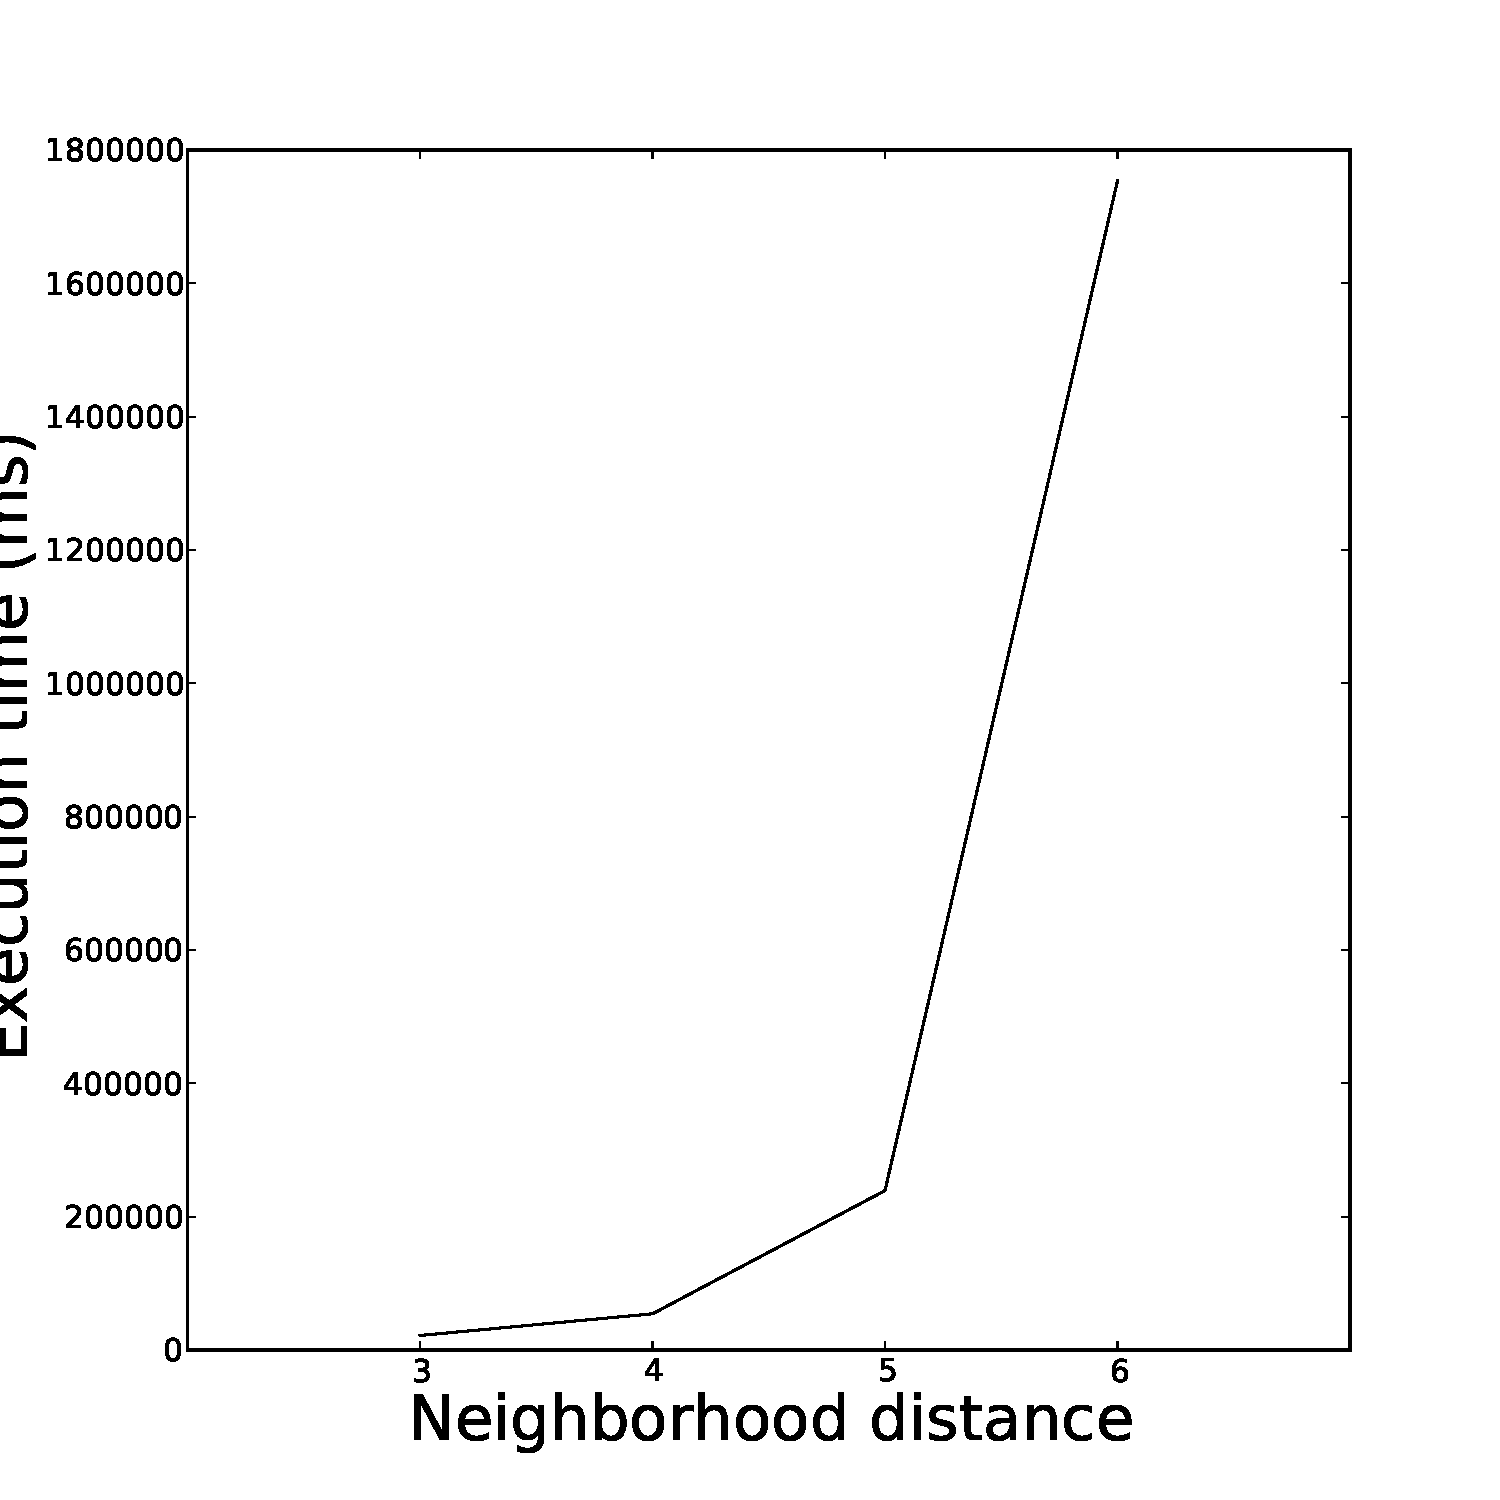
\includegraphics[width=5cm,height=5cm]{image/win_2_rank_2.pdf}}	
			\end{subfigure}
			\begin{subfigure}[rank = 3]
					{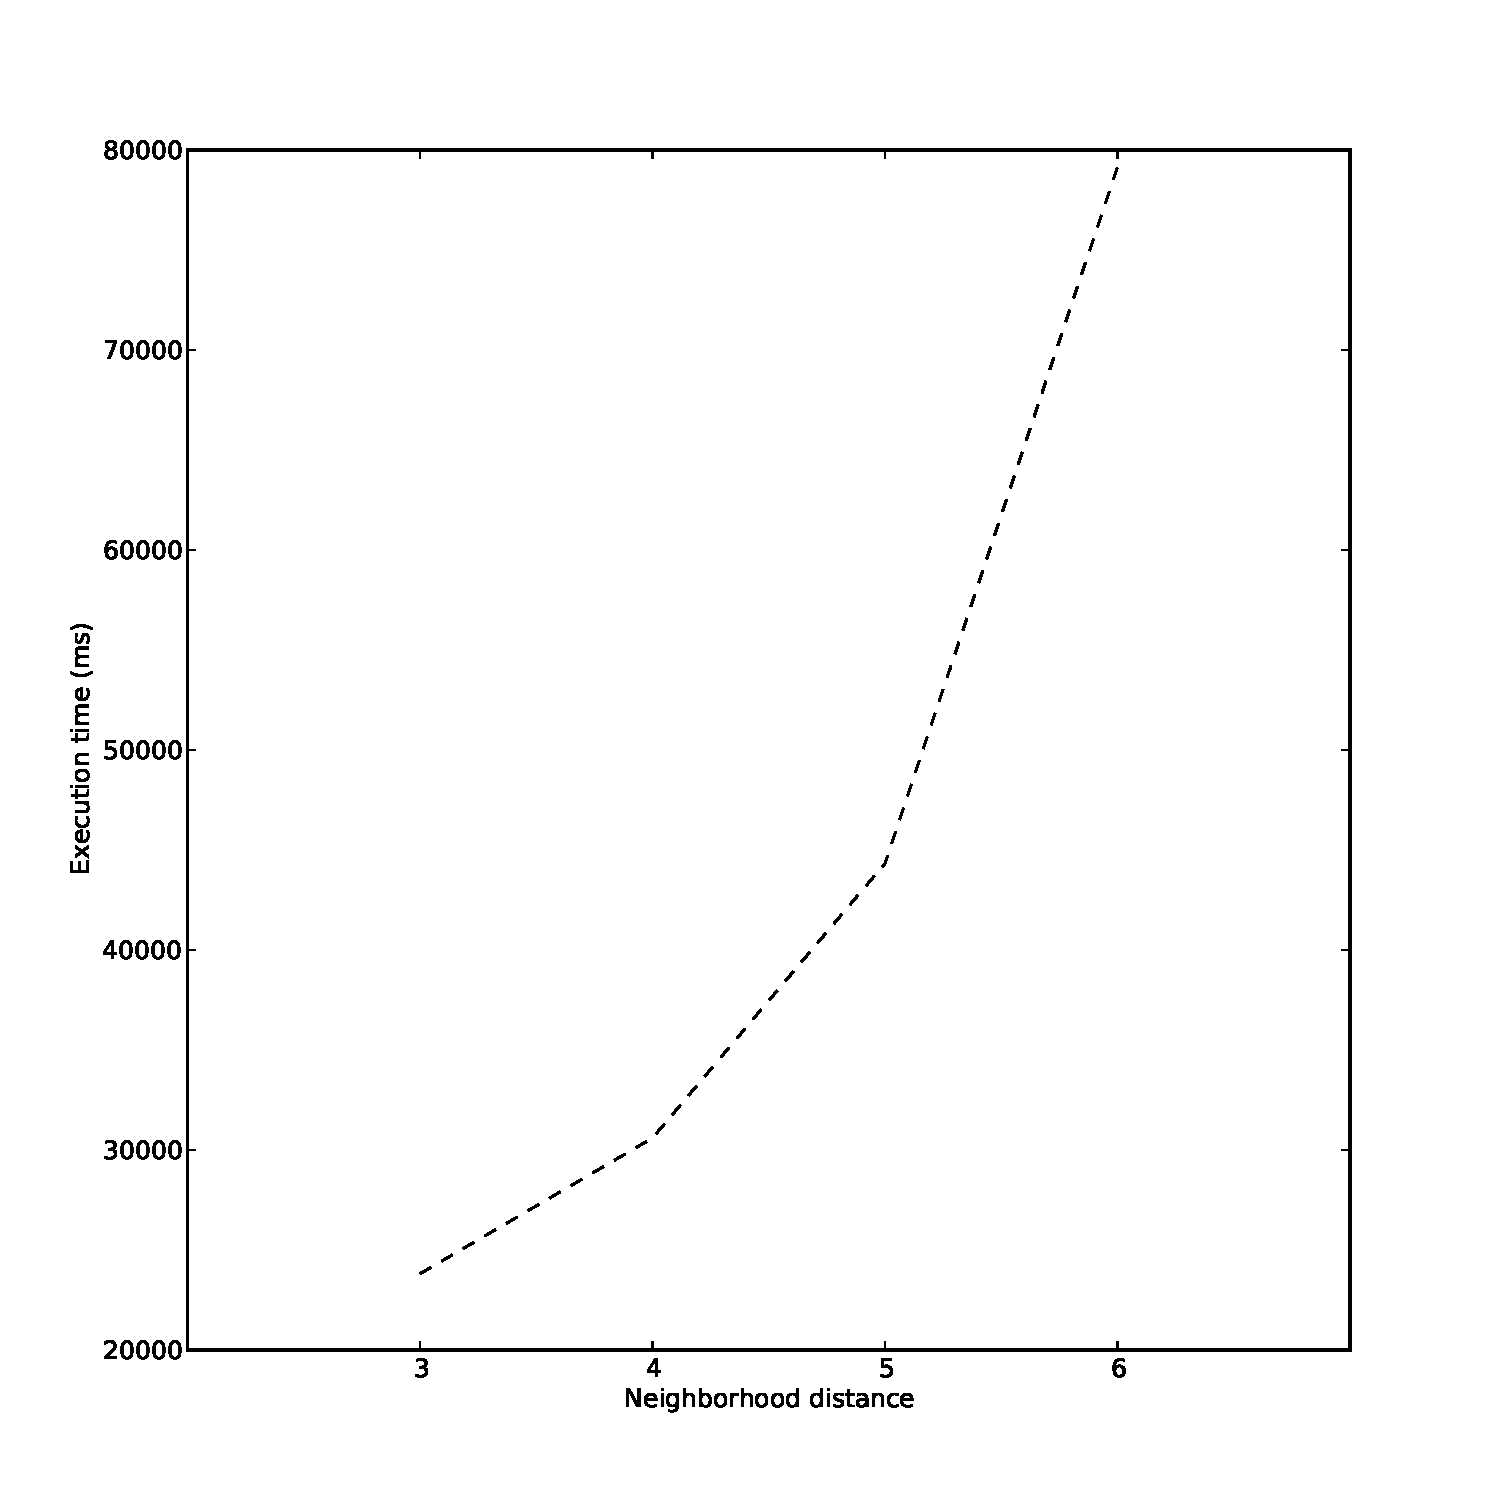
\includegraphics[width=5cm,height=5cm]{image/win_2_rank_3.pdf}}	
			\end{subfigure}
			\begin{subfigure}[rank = 4]
					{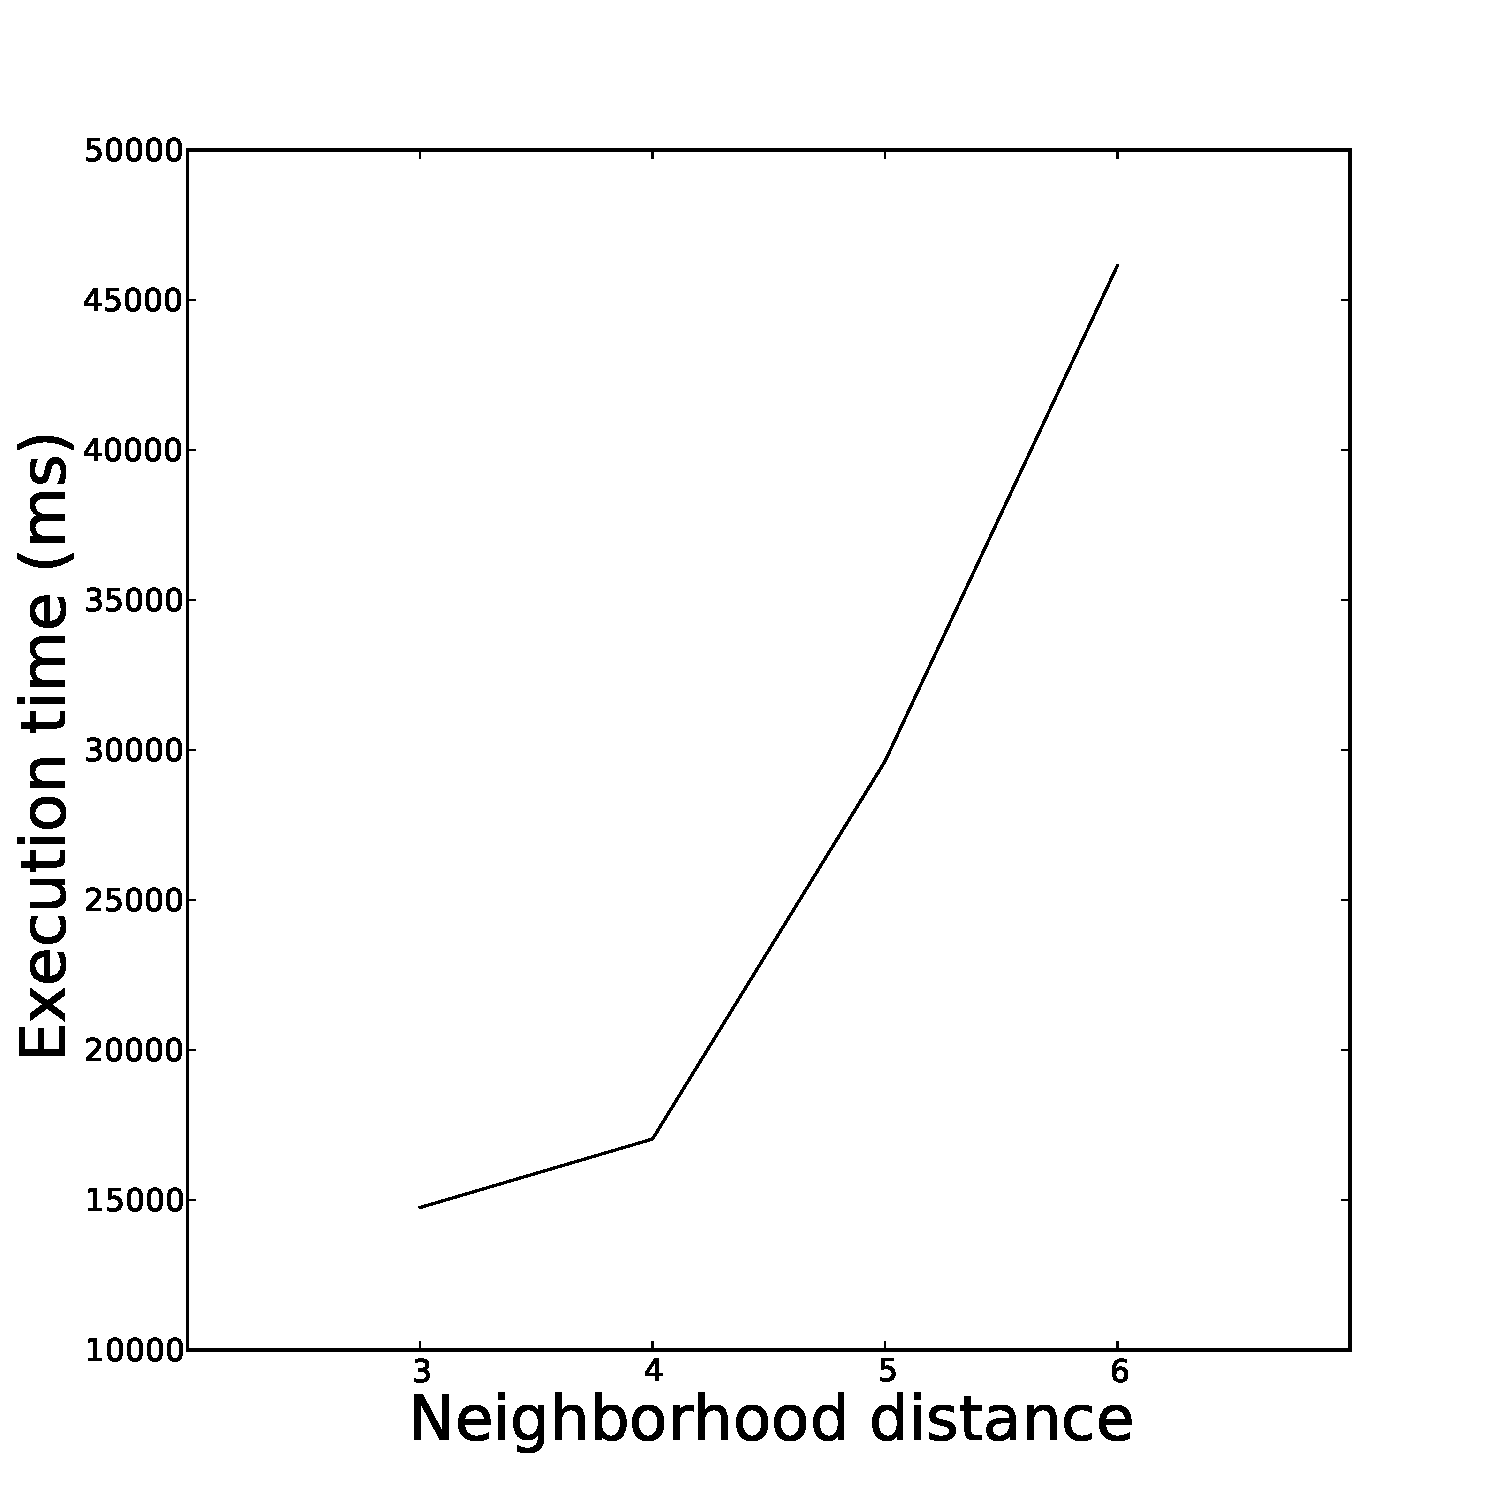
\includegraphics[width=5cm,height=5cm]{image/win_2_rank_4.pdf}}	
			\end{subfigure}
			\caption[et-fixed-10days-r-rank]{Execution time for different rank value}
	\label{fig:et-fixed-10days-r-rank}
\end{figure*} 

In figure \ref{fig:et-fixed-10days-r-nd} is possible to see how the computation time change respect to the rank value at different neighbourhood distance. 
Surprisingly for a neighbourhood distance = 3 the computation time with a n-gram graph of rank=3 is slightly higher respect to a rank=2. 
That is quite strange since slicing a text in two-gram should produce more node that slicing a text in three-grams.
Probably with rank = 2 and ND = 3; near grams are part of the same word creating graph easy to compute.
This scenario produce a smaller computation time in a two-gram graph that a three-gram graph where we have more distinct node and so edge to check.

Is possible to notice how for bigger ND values, the computation time for of the 2-gram diverge, instead 3-gram became more similar at the 4-gram behaviour. Probably because computing the similarity between 2-gram graph is an operation quite expensive since they have many edges to check.

\begin{figure*}[htbp]
	\centering
			\begin{subfigure}[neighbourhood distance = 3]
					{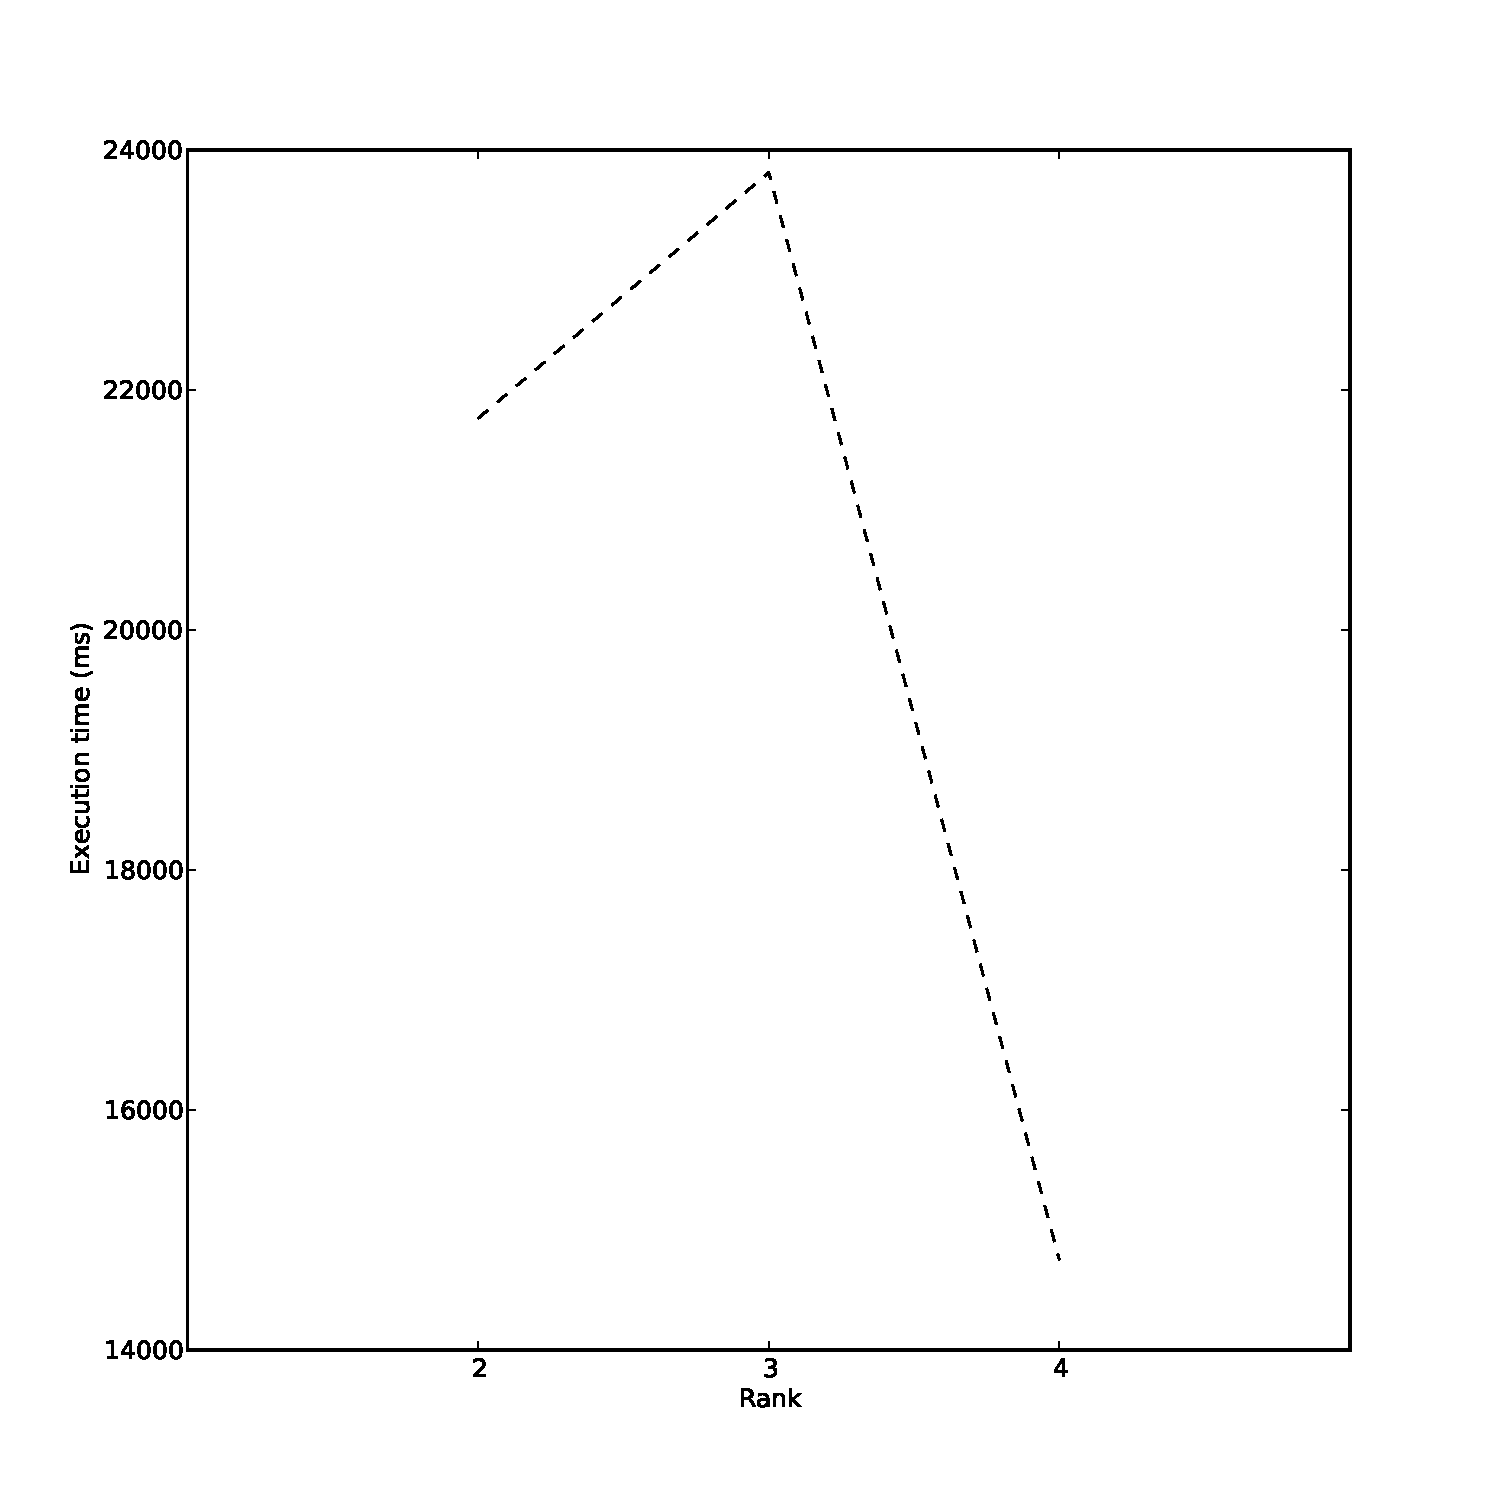
\includegraphics[width=5cm,height=5cm]{image/win_2_ndist_3.pdf}}	
			\end{subfigure}
			\begin{subfigure}[neighbourhood distance = 4]
					{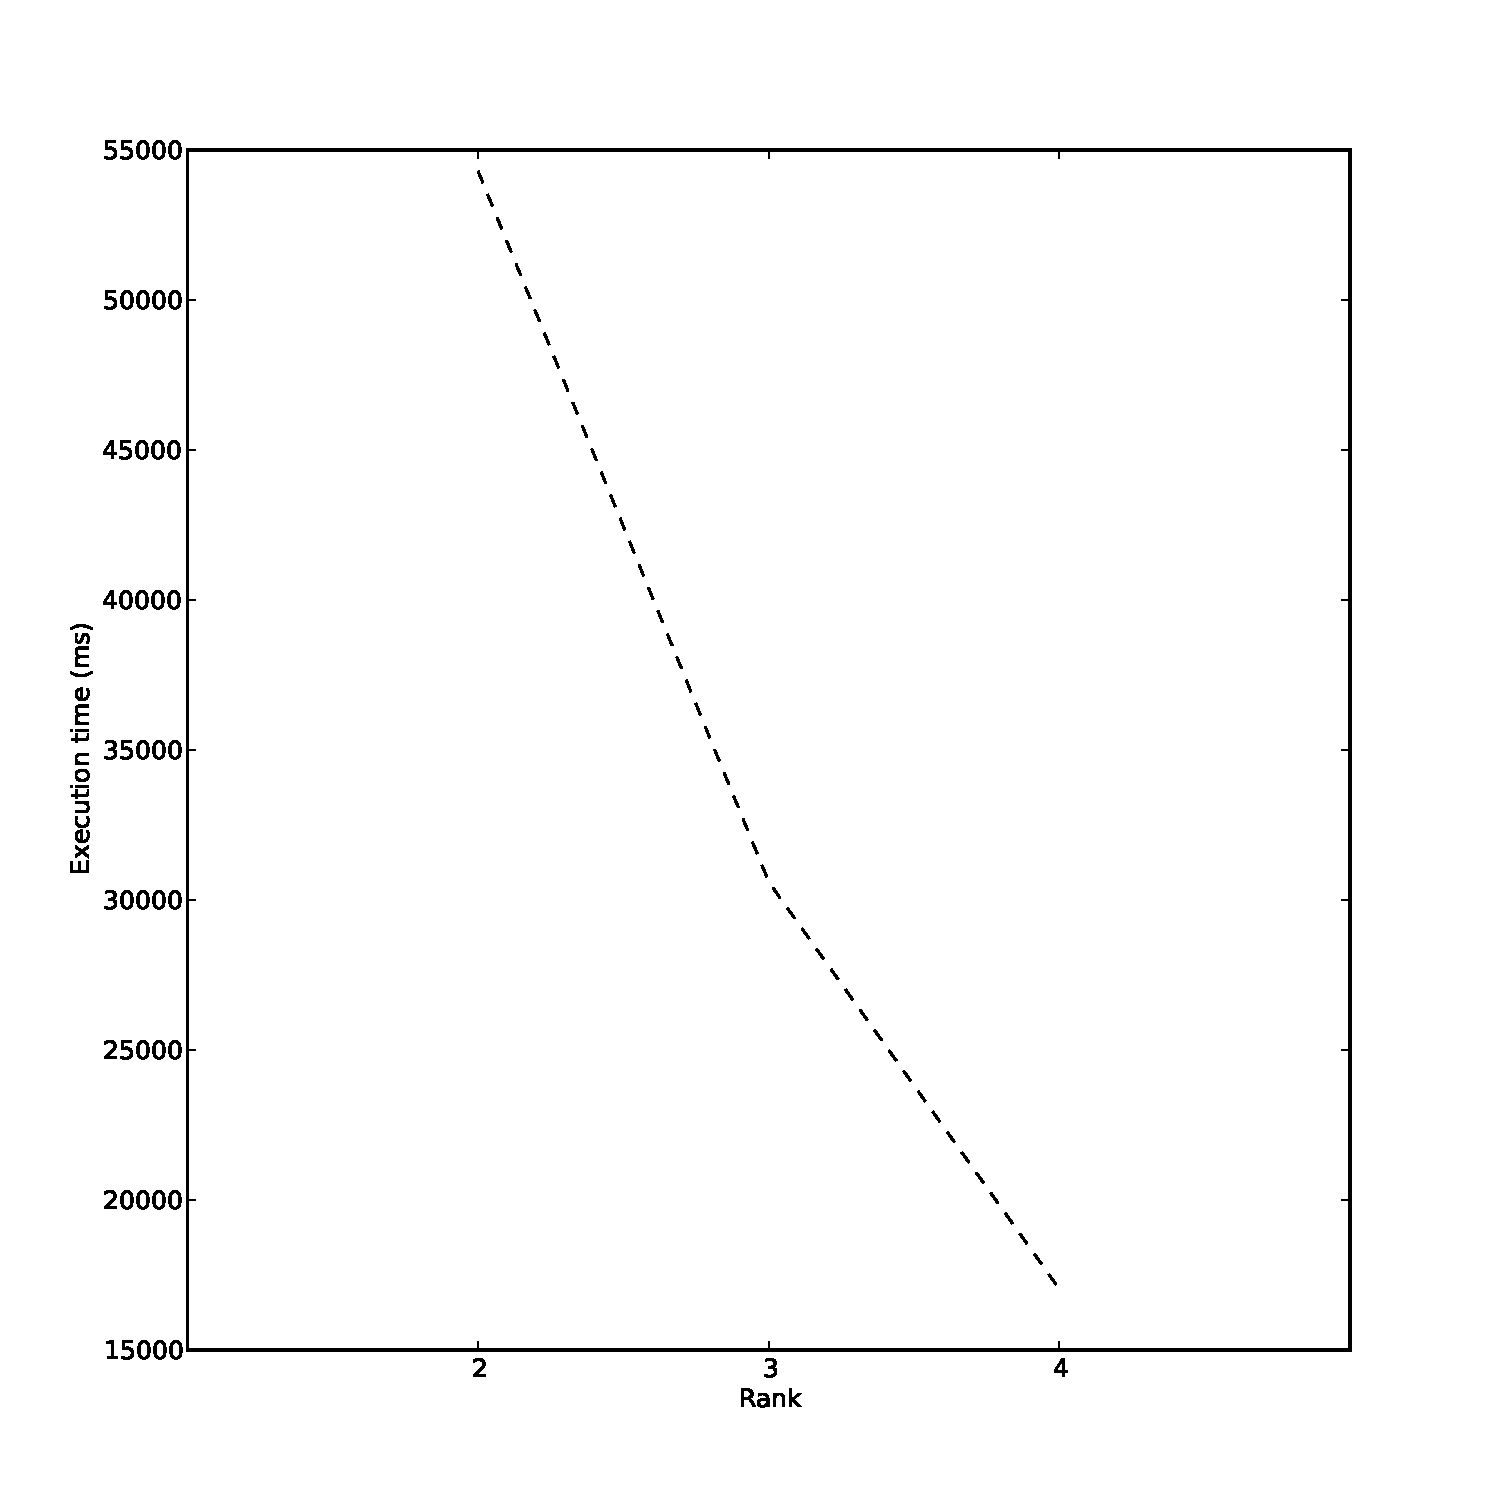
\includegraphics[width=5cm,height=5cm]{image/win_2_ndist_4.pdf}}	
			\end{subfigure}
			\begin{subfigure}[neighbourhood distance = 5]
					{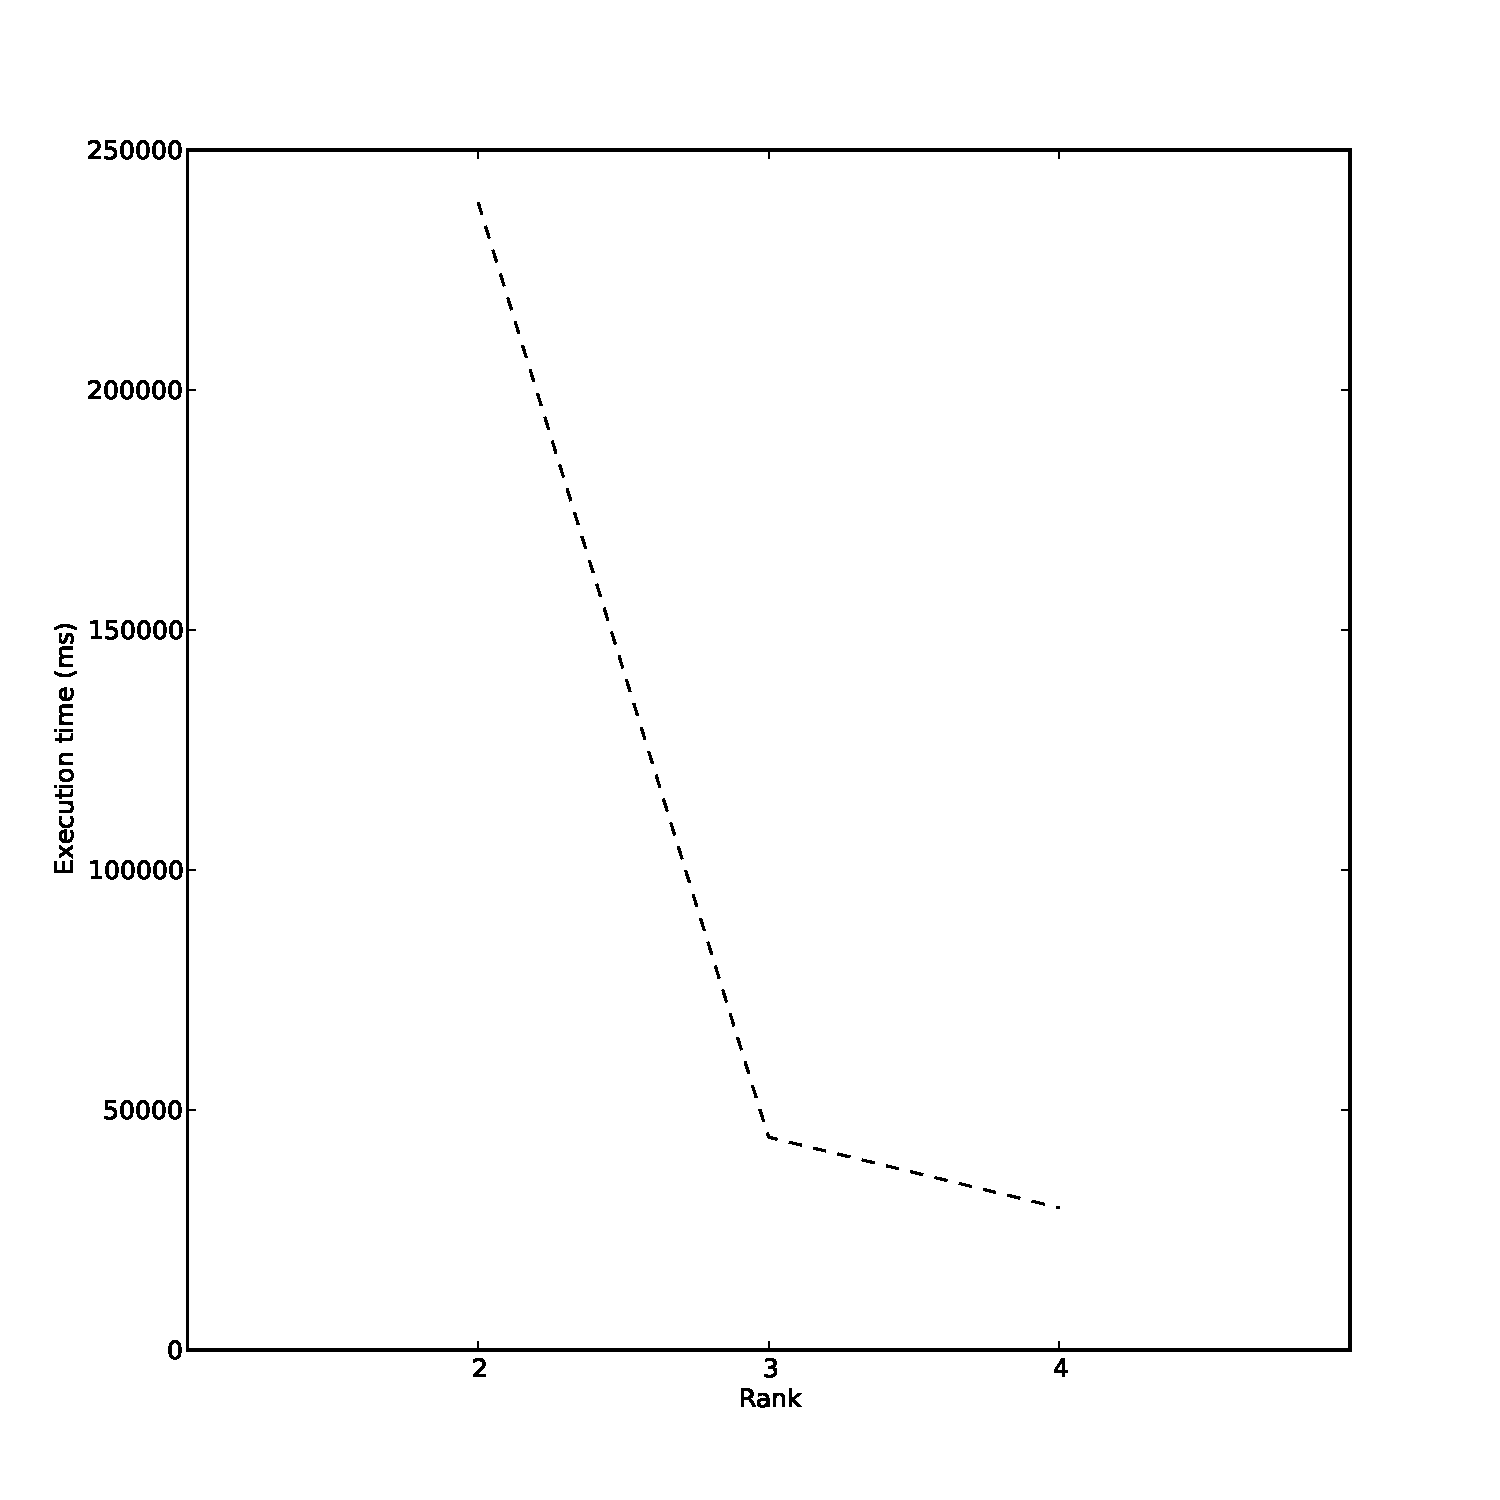
\includegraphics[width=5cm,height=5cm]{image/win_2_ndist_5.pdf}}	
			\end{subfigure}
			\begin{subfigure}[neighbourhood distance = 6]
					{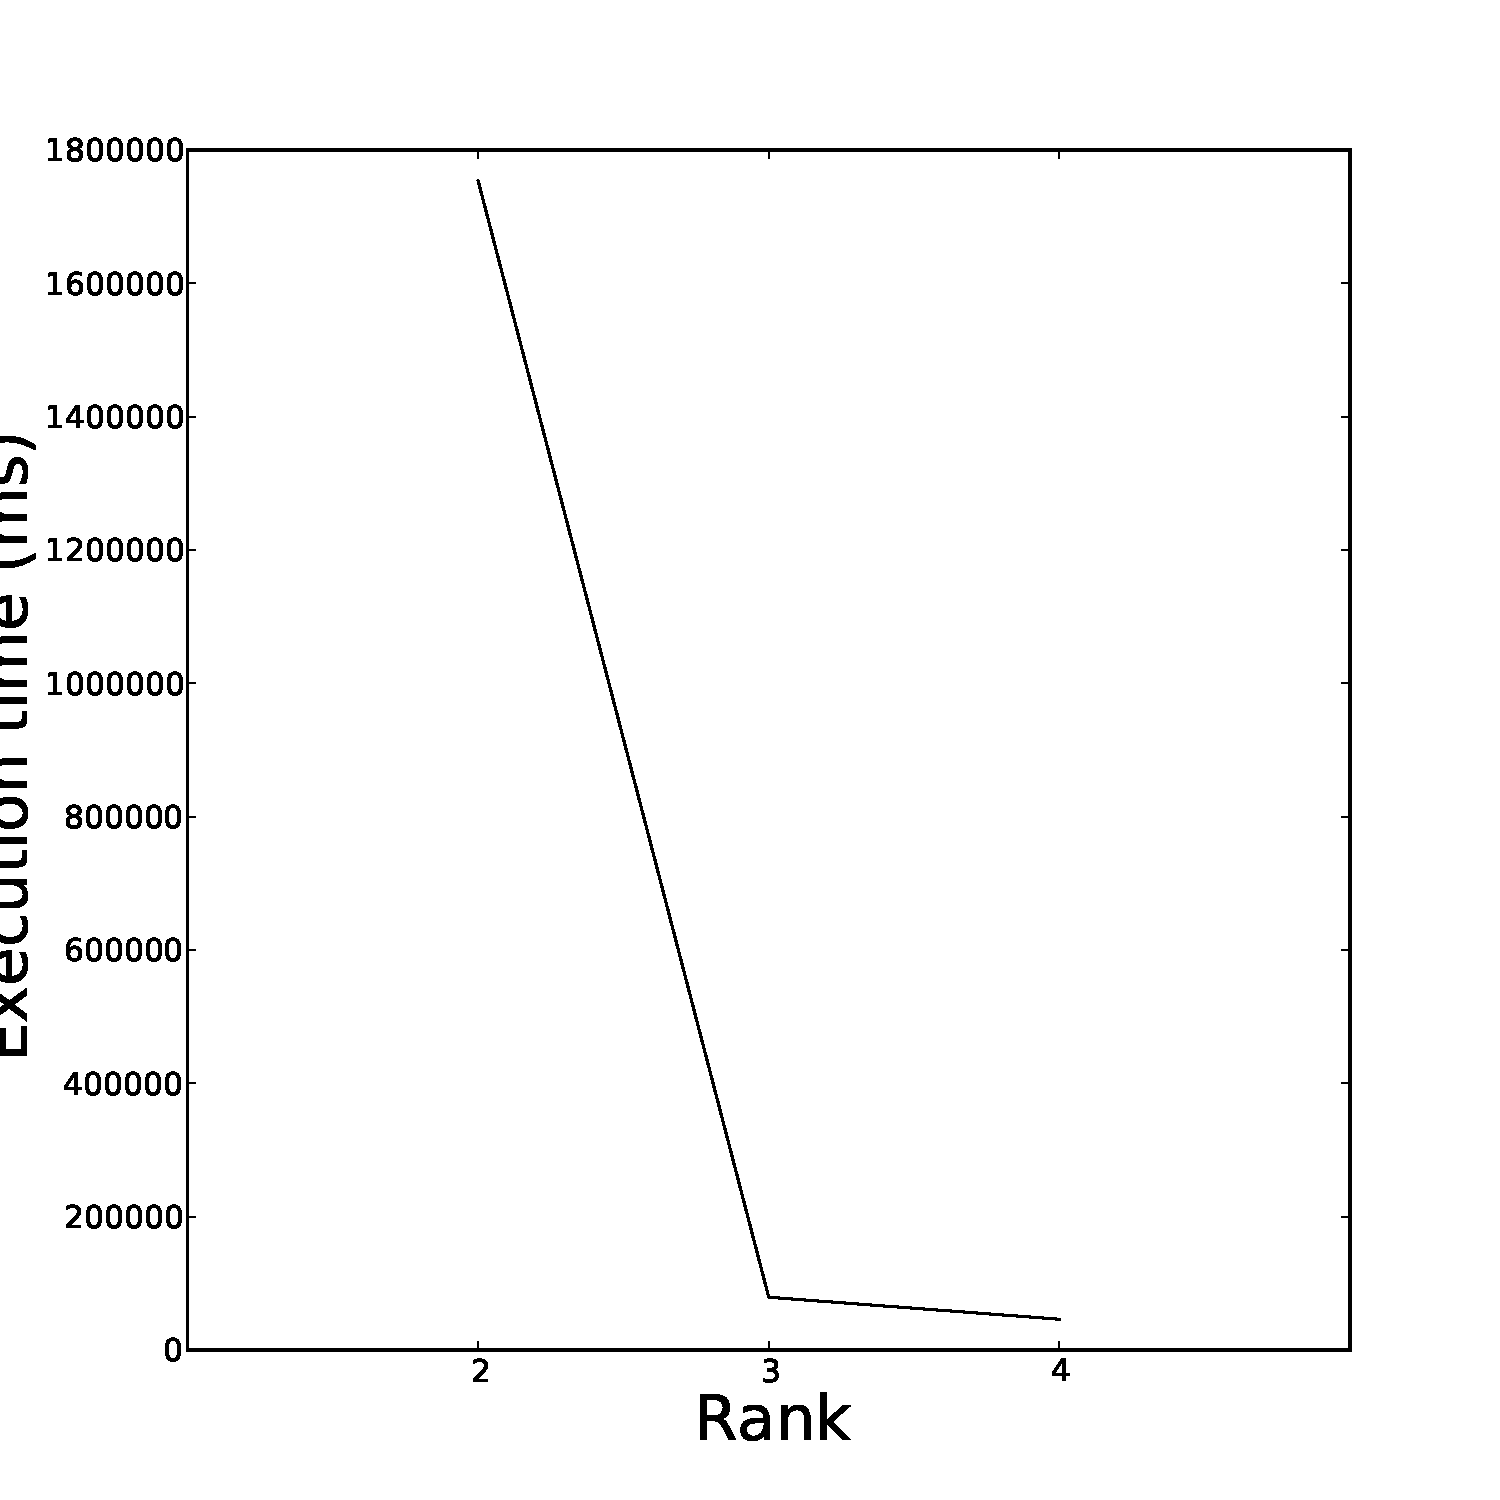
\includegraphics[width=5cm,height=5cm]{image/win_2_ndist_6.pdf}}	
			\end{subfigure}
			\caption[et-fixed-10days-r-nd]{Execution time for different neighbourhood distance }
	\label{fig:et-fixed-10days-r-nd}
\end{figure*} 


%Figure \ref{fig:et-fixed-r3-winds} report the variation of computation time for fixed rank value(3). The shape of the computation time in this case is always the same: exponential respect the ND. 
%Notice that the max computation time always increase with the increasing of the windows size, since the algorithm have to compute the similarity between more news. In this way we can derive that the number of news, inside the time windows, affect the computation time in a almost linear way.


